\section{Rozkład Cholesky’ego}
Macierz C jest \textbf{dodatnio określona}, jeśli \( \forall_x\; x^TCx > 0 \). \\
Macierz C jest \textbf{dodatnio półokreślona}, jeśli \( \forall_x\; x^TCx \geq 0 \). \\
Dla każdej macierzy \( A \), macierz \( A^TA \) jest dodatnio półokreślona, a jeśli kolumny \( A \) są liniowo niezależne, to jest dodatnio określona. Do tego jest symetryczna. Można ją więc rozłożyć na \( LL^T \), rozkład Cholesky'ego:
\begin{multicols}{2}
\noindent
Już wyliczone: \( L_{1,1}, \dots, L_{i,1}, \dots, L_{i, j-1} \) \\
\( A_{ij} = L_i \cdot L_j = \sum_{k=1}^{j}\; L_{ik}L_{jk} \) \\
\( L_{ij} = \frac{A_{ij} - \sum_{k=1}^{j-1}\; L_{ik}L_{jk}}{L_{jj}}, \text{ dla } i > j \) \\
\( L_{ii} = \sqrt{A_{ii} - \sum_{k=1}^{i-1}\; L_{ik}^2} \) \\
\columnbrake
czyli takim zygzakiem.
\begin{figure}[H]
    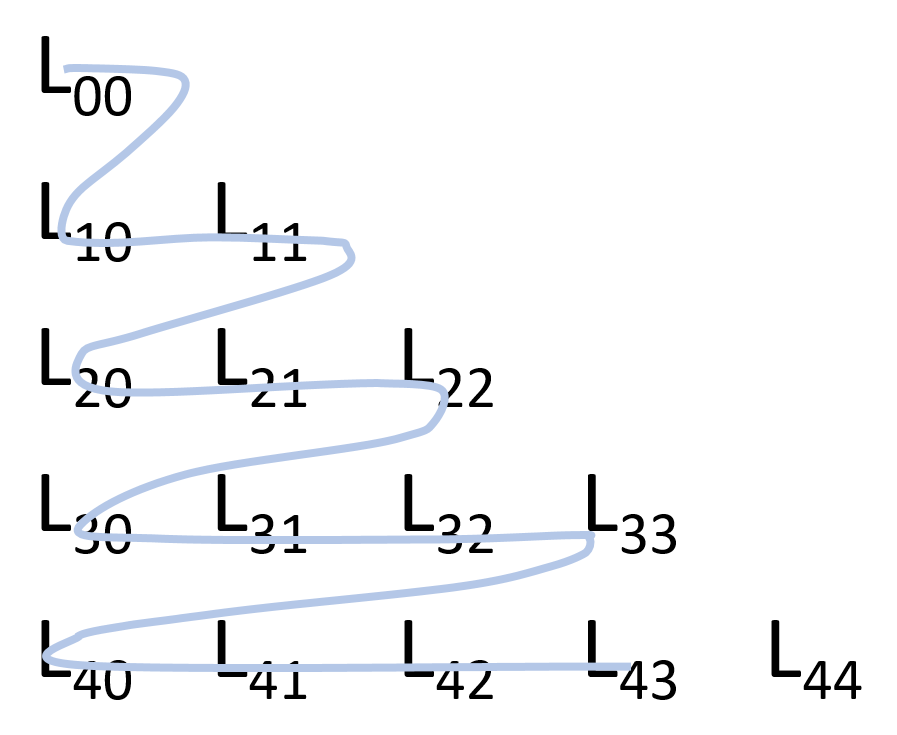
\includegraphics[width=0.21\textwidth]{img/cholesky.png}
\end{figure}
\end{multicols}
\noindent
Rozkład Cholesky’ego jest stabilniejszy numerycznie i ma lepszą stałą niż standardowa eliminacja Gaussa.